\documentclass{article}

\usepackage{hyperref}
\hypersetup{
	colorlinks=true,
	linkcolor=blue,
	urlcolor=cyan,}
\usepackage{booktabs}
\usepackage{textgreek}

%%%%%%%%%%%%%%%%%%%%%%%%%%%%%%%%%%%%%%%%%
% Lachaise Assignment
% Structure Specification File
% Version 1.0 (26/6/2018)
%
% This template originates from:
% http://www.LaTeXTemplates.com
%
% Authors:
% Marion Lachaise & François Févotte
% Vel (vel@LaTeXTemplates.com)
%
% License:
% CC BY-NC-SA 3.0 (http://creativecommons.org/licenses/by-nc-sa/3.0/)
% 
%%%%%%%%%%%%%%%%%%%%%%%%%%%%%%%%%%%%%%%%%

%----------------------------------------------------------------------------------------
%	PACKAGES AND OTHER DOCUMENT CONFIGURATIONS
%----------------------------------------------------------------------------------------

\usepackage{amsmath,amsfonts,stmaryrd,amssymb} % Math packages

\usepackage{enumerate} % Custom item numbers for enumerations

\usepackage[ruled]{algorithm2e} % Algorithms

\usepackage[framemethod=tikz]{mdframed} % Allows defining custom boxed/framed environments

\usepackage{listings} % File listings, with syntax highlighting
\lstset{
	basicstyle=\ttfamily, % Typeset listings in monospace font
}

%----------------------------------------------------------------------------------------
%	DOCUMENT MARGINS
%----------------------------------------------------------------------------------------

\usepackage{geometry} % Required for adjusting page dimensions and margins

\geometry{
	paper=a4paper, % Paper size, change to letterpaper for US letter size
	top=2.5cm, % Top margin
	bottom=3cm, % Bottom margin
	left=2.5cm, % Left margin
	right=2.5cm, % Right margin
	headheight=14pt, % Header height
	footskip=1.5cm, % Space from the bottom margin to the baseline of the footer
	headsep=1.2cm, % Space from the top margin to the baseline of the header
	%showframe, % Uncomment to show how the type block is set on the page
}

%----------------------------------------------------------------------------------------
%	FONTS
%----------------------------------------------------------------------------------------

\usepackage[utf8]{inputenc} % Required for inputting international characters
\usepackage[T1]{fontenc} % Output font encoding for international characters

\usepackage{XCharter} % Use the XCharter fonts

%----------------------------------------------------------------------------------------
%	COMMAND LINE ENVIRONMENT
%----------------------------------------------------------------------------------------

% Usage:
% \begin{commandline}
%	\begin{verbatim}
%		$ ls
%		
%		Applications	Desktop	...
%	\end{verbatim}
% \end{commandline}

\mdfdefinestyle{commandline}{
	leftmargin=10pt,
	rightmargin=10pt,
	innerleftmargin=15pt,
	middlelinecolor=black!50!white,
	middlelinewidth=2pt,
	frametitlerule=false,
	backgroundcolor=black!5!white,
	frametitle={Command Line},
	frametitlefont={\normalfont\sffamily\color{white}\hspace{-1em}},
	frametitlebackgroundcolor=black!50!white,
	nobreak,
}

% Define a custom environment for command-line snapshots
\newenvironment{commandline}{
	\medskip
	\begin{mdframed}[style=commandline]
}{
	\end{mdframed}
	\medskip
}

%----------------------------------------------------------------------------------------
%	FILE CONTENTS ENVIRONMENT
%----------------------------------------------------------------------------------------

% Usage:
% \begin{file}[optional filename, defaults to "File"]
%	File contents, for example, with a listings environment
% \end{file}

\mdfdefinestyle{file}{
	innertopmargin=1.6\baselineskip,
	innerbottommargin=0.8\baselineskip,
	topline=false, bottomline=false,
	leftline=false, rightline=false,
	leftmargin=2cm,
	rightmargin=2cm,
	singleextra={%
		\draw[fill=black!10!white](P)++(0,-1.2em)rectangle(P-|O);
		\node[anchor=north west]
		at(P-|O){\ttfamily\mdfilename};
		%
		\def\l{3em}
		\draw(O-|P)++(-\l,0)--++(\l,\l)--(P)--(P-|O)--(O)--cycle;
		\draw(O-|P)++(-\l,0)--++(0,\l)--++(\l,0);
	},
	nobreak,
}

% Define a custom environment for file contents
\newenvironment{file}[1][File]{ % Set the default filename to "File"
	\medskip
	\newcommand{\mdfilename}{#1}
	\begin{mdframed}[style=file]
}{
	\end{mdframed}
	\medskip
}

%----------------------------------------------------------------------------------------
%	NUMBERED QUESTIONS ENVIRONMENT
%----------------------------------------------------------------------------------------

% Usage:
% \begin{question}[optional title]
%	Question contents
% \end{question}

\mdfdefinestyle{question}{
	innertopmargin=1.2\baselineskip,
	innerbottommargin=0.8\baselineskip,
	roundcorner=5pt,
	nobreak,
	singleextra={%
		\draw(P-|O)node[xshift=1em,anchor=west,fill=white,draw,rounded corners=5pt]{%
		Question \theQuestion\questionTitle};
	},
}

\newcounter{Question} % Stores the current question number that gets iterated with each new question

% Define a custom environment for numbered questions
\newenvironment{question}[1][\unskip]{
	\bigskip
	\stepcounter{Question}
	\newcommand{\questionTitle}{~#1}
	\begin{mdframed}[style=question]
}{
	\end{mdframed}
	\medskip
}

%----------------------------------------------------------------------------------------
%	WARNING TEXT ENVIRONMENT
%----------------------------------------------------------------------------------------

% Usage:
% \begin{warn}[optional title, defaults to "Warning:"]
%	Contents
% \end{warn}

\mdfdefinestyle{warning}{
	topline=false, bottomline=false,
	leftline=false, rightline=false,
	nobreak,
	singleextra={%
		\draw(P-|O)++(-0.5em,0)node(tmp1){};
		\draw(P-|O)++(0.5em,0)node(tmp2){};
		\fill[black,rotate around={45:(P-|O)}](tmp1)rectangle(tmp2);
		\node at(P-|O){\color{white}\scriptsize\bf !};
		\draw[very thick](P-|O)++(0,-1em)--(O);%--(O-|P);
	}
}

% Define a custom environment for warning text
\newenvironment{warn}[1][Warning:]{ % Set the default warning to "Warning:"
	\medskip
	\begin{mdframed}[style=warning]
		\noindent{\textbf{#1}}
}{
	\end{mdframed}
}

%----------------------------------------------------------------------------------------
%	INFORMATION ENVIRONMENT
%----------------------------------------------------------------------------------------

% Usage:
% \begin{info}[optional title, defaults to "Info:"]
% 	contents
% 	\end{info}

\mdfdefinestyle{info}{%
	topline=false, bottomline=false,
	leftline=false, rightline=false,
	nobreak,
	singleextra={%
		\fill[black](P-|O)circle[radius=0.4em];
		\node at(P-|O){\color{white}\scriptsize\bf i};
		\draw[very thick](P-|O)++(0,-0.8em)--(O);%--(O-|P);
	}
}

% Define a custom environment for information
\newenvironment{info}[1][Info:]{ % Set the default title to "Info:"
	\medskip
	\begin{mdframed}[style=info]
		\noindent{\textbf{#1}}
}{
	\end{mdframed}
}
 % Include the file specifying the document structure and custom commands

%----------------------------------------------------------------------------------------
%	ASSIGNMENT INFORMATION
%----------------------------------------------------------------------------------------

\title{Week 5: Electrocardiography (EEG)}
\author{BIOE 320 Systems Physiology Laboratory} 
\date{}
%----------------------------------------------------------------------------------------

\begin{document}
\large
\maketitle

\section*{Objectives}
\begin{enumerate}
	\item To become familiar with the ECG as a primary tool for evaluating electrical events within the heart
	\item To correlate electrical events as displayed on the ECG with the mechanical events that occur during the cardiac cycle
	\item To observe rate and rhythm changes in the ECG associated with the body position and breathing
	\item To observe the effects of changing ECG sampling rate on the ECG recordings
\end{enumerate}

\section*{Background}
The heart is the physiological engine of the circulatory system, receiving blood from veins and pumping it into arteries. The contractions of myocardium (heart tissue) are a result of electrical signals that originate in the sinoatrial (SA) node of the heart. The SA node acts as a pacemaker for the rest of the heart, keeping a constant rhythm. Based on changing physiological demands, the frequency of impulses can be sped up or slowed down by extrinsic motor nerves via sympathetic and parasympathetic pathways, respectively.

\subsection*{Electrical Pathways}
\begin{figure}[h]
\centering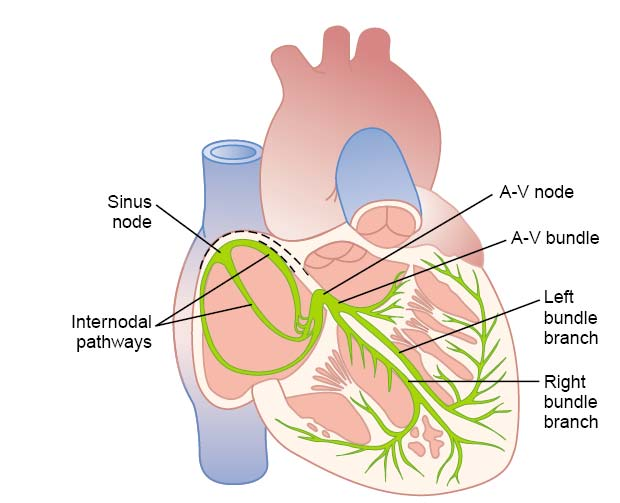
\includegraphics[width=0.5\textwidth]{../images/ECG_I_1.jpg}
\caption{Schematic of the cardiac conduction system}
\label{pathways}
\end{figure}
Electrical impulses (Fig. \ref{pathways}) proceed from the SA node, causing atrial muscles to contract by producing an action potential (depolarization). The signal is then conducted to the atrioventricular (AV) node, which lies between the right atrium and ventricle. After a short delay to allow blood to flow out of the atria and into the ventricles, the AV node relays the electrical signal to the bundle of His where the signal splits between the right and left bundle branches. These branches continue to subdivide into Purkinje fibers, which pass on the action potential to ventricular muscle, stimulating the ventricles to contract. After depolarization takes place, subsequent repolarization occurs in which cardiac cells return to their resting state and the cardiac muscles relax.

\subsection*{Electrocardiogram}
The electric currents that travel through the heart can be picked up on the surface of the body in the form of electrical potential. Plotted against time, these readings are known as an electrocardiogram (ECG, seen in Fig. \ref{ecg}).\\

\begin{figure}[h]
\centering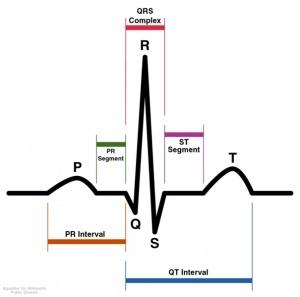
\includegraphics[width=0.6\textwidth]{../images/ECG_I_2.jpg}
\caption{Schematic of an electrocardiogram}
\label{ecg}
\end{figure}

There are many different ways to place the electrodes to measure an ECG signal. In the lab today, we will use standard bipolar leads, in which 2 electrodes (positive and negative) are located on different sides of the heart and are measured against a common ground (third electrode).\\

The baseline of the ECG is known as the isoelectric line. The first peak, called the P wave, correlates to depolarization of the atrial muscle. The QRS system represents both the depolarization of the ventricular muscle as well as repolarization of the atrial muscle. Finally, the T wave correlates to the repolarization of the ventricles.\\

The PR interval is measured from the beginning of the P wave to the beginning of the QRS complex. Physiologically, it represents the time interval between atrial and ventricular depolarization. An abnormally long PR interval suggests conduction problems between the SA node and AV node. The QT interval is measured from the Q wave to the end of the T wave and is also known as ventricular systole, or period of ventricular contraction. Ventricular diastole is the period from the end of the T wave to the peak of the P wave. Finally, the period of atrial contraction, or atrial systole, is measured from the peak of the P wave to the Q wave.

\section*{Required Supplies}
\begin{itemize}
	\item BIOPAC student labs lesson L05: ECG I
	\item BIOPAC MP3X data acquisition unit
	\item BIOPAC electrode lead set
	\item BIOPAC disposable vinyl electrodes
	\item Optional but useful: alcohol wipes, abrasive pads, physiology tape, electrode gel
\end{itemize}

\section*{Setting Up}
\begin{enumerate}
	\item Turn on the MP3X acquisition unit by flipping the switch found on the back panel.
	\item Place electrodes and leads on the subject as follows (Fig. \ref{ecg}):\begin{itemize}
		\item Positive (red): inside of left ankle, just above the ankle bone
		\item Negative (white): inside of the right wrist
		\item Ground (black): right ankle bone
	\end{itemize}
	\begin{figure}[h]
	\centering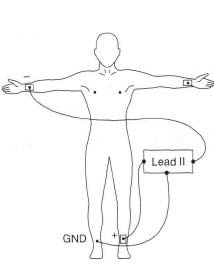
\includegraphics[width=0.4\textwidth]{../images/ECG_I_3.jpg}
	\caption{Schematic of electrode lead placement}
	\label{ecg}
	\end{figure}
	
	\item Plug the electrode cord, SS2L, into channel 2 and connect to the electrodes.
	\item Open Biopac Pro v3.7 (\textbf{not the student lessons})
	\item Go under the MP3X pull-down menu and select Set-up Acquistion (Fig. \ref{setup}).
	\begin{figure}[h]
	\centering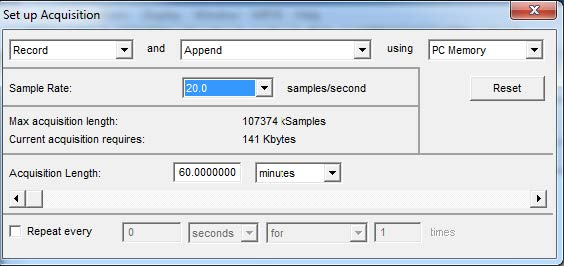
\includegraphics[width=0.6\textwidth]{../images/ECG_I_4.jpg}
	\caption{Set-up acquisition window}
	\label{setup}
	\end{figure}
	
	\item Set the sampling rate to 20/sec. Click reset and close the box.
	\item Go under the MP3X pull-down menu and select Set-up Channels (Fig. \ref{setup_2}).
	\begin{figure}[h]
	\centering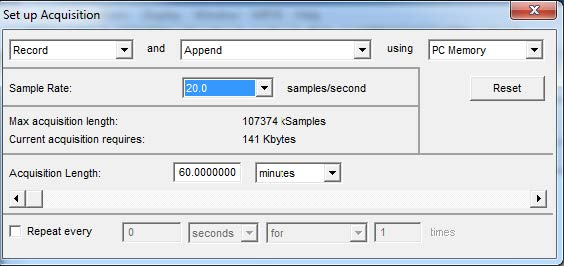
\includegraphics[width=0.6\textwidth]{../images/ECG_I_4.jpg}
	\caption{Set-up channels}
	\label{setup_2}
	\end{figure}
	
	\item Under the presets drop-down arrow, select ECG 0.05 Hz - 150 Hz for both channels 1 and 3.
	\item Check all 3 boxes for channel 2. Deselect all boxes for channels 1 and 3.
	\item Take a sample 30 sec ECG recording by pressing Start.
\end{enumerate}

\subsection*{Changing Sampling Rate}
\begin{enumerate}
	\item Go under the MP3X pull-down menu and select Set-Up Acquisition (Fig. \ref{setup}).
	\item Set the sampling rate to 200/sec.
	\item Take another 30 sec ECG recording by pressing Start.
	\item Close BIOPAC Pro Software. Do NOT remove electrodes or leads from the subject.
	\item What are the differences between the recordings at 20 Hz and 200 Hz?
	\item What criteria should be used to establish an appropriate sampling rate?
\end{enumerate}

\section*{Experiments}
\subsection*{Setting Up}
\begin{enumerate}
	\item Plug the electrode cord into channel 1 and connect the electrodes.
	\item Launch the BIOPAC software by clicking on the BSL Lessons 3.7.6 icon and select L05-ECG-1 as shown in Fig. \ref{lesson}.
		
		\begin{figure}[h]
	\centering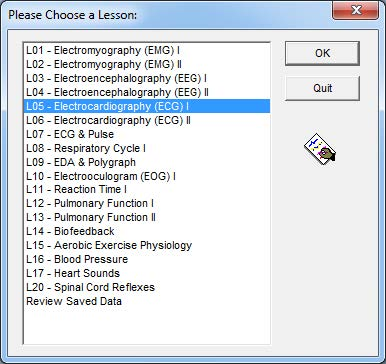
\includegraphics[width=0.6\textwidth]{../images/ECG_I_6.jpg}
		\caption{Selecting BIOPAC lesson L05-ECG-I}
		\label{lesson}
		\end{figure}
\end{enumerate}

\subsection*{Calibration}
\begin{info}
	The calibration procedure establishes the hardware's internal parameters (such as gain, offset, and scaling) and is critical for optimum performance. Pay close attention to the calibration procedure.
\end{info}
\begin{enumerate}
	\item Check that electrodes are still adhered to the skin, If they are being pulled up, you will not get a good ECG signal. The subject must be relaxed and as still as possible during the calibration procedure. The ECG is very sensitive to small changes in voltage caused by contraction of skeletal muscles, so the subject's arms and legs need to be relaxed so that the muscle (EMG) signal does not corrupt the ECG signal.
	\item Click on Calibrate. The calibration procedure will begin and then stop automatically after 8 seconds. At the end of the calibration recording, the screen should resemble Fig. \ref{calibration} below. There should be a regular, periodic ECG waveform with a relatively flat baseline. Some tips for obtaining optimal data:\begin{itemize}
		\item The subject should not talk or laugh during any of the recording segments.
		\item The subject should be in a relaxed state for each recording segment and in the position noted for each segment.
		\item When the subject is asked to sit up, they should do so in a chair, with arms relaxed.
		\end{itemize}
		
		\begin{figure}[h]
	\centering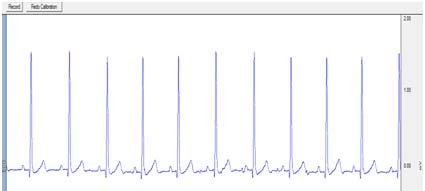
\includegraphics[width=0.6\textwidth]{../images/ECG_I_7a.jpg}
	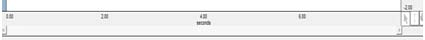
\includegraphics[width=0.6\textwidth]{../images/ECG_I_7b.jpg}
		\caption{Example calibration}
		\label{calibration}
		\end{figure}
		
	\item If the data recording shows any jitter or large baseline drifts, you should redo the calibration by clicking on the Redo Calibration button.
\end{enumerate}

\subsection*{Segment 1: Supine (Laying Down)}
\begin{enumerate}
	\item Prepare for the recording by having the subject lie down and relax with their eyes closed.
	\item Click on Record, and record data for 20 seconds, then click on Suspend at the 20 second mark. Proceed unless:
		\begin{itemize}
			\item The suspend button was pressed prematurely.
			\item An electrode peeled up, causing a large baseline drift, spike, or loss of signal.
			\item The subject has too much muscle (EMG) artifact.
		\end{itemize}
\end{enumerate}

\subsection*{Segment 2: Sitting Up}
\begin{enumerate}
	\item Starting from the supine position, have the subject sit up quickly. Click on Resume and record for another 20 seconds. The recording will continue from the point where it last stopped and a marker labeled "sitting up" will automatically come up when Resume is pressed.\begin{info}
In order to capture the heart rate variation, it is important that you click on Resume to continue recording as quickly as possible after the subject sits up. However, it is also important that you do not click on Resume while the subject is \textit{in the process of} sitting up or you will capture motion artifact.	
\end{info}

	\item Click on Suspend at the end of the 20 second recording segment (at the 40 second mark total). Proceed unless you see any of the conditions described in Segment 1.
\end{enumerate}

\subsection*{Segment 3: Deep Breaths}
\begin{enumerate}
	\item Click on Resume. The recording will continue from the point where it last stopped, and a marker labeled "5 deep breaths" will automatically come up when Resume is pressed.
	\item Record for 20 seconds and have the subject take in 5 deep breaths during recording. The 5 deep breathing cycles should be deeper and slower than normal breathing at rest and should follow one another.
	\item During this time, the person operating the software should insert a marker at the beginning of an inhale and insert another marker at the corresponding exhale. The recorder should label these markers "inhale" and "exhale" (note: the hotkey for a marker is F9).
	\item At the end of the 20 second recording segment, click on Suspend. Note that deep breathing may produce a baseline drift. This is normal and does not necessitate redoing the recording.
\end{enumerate}

\subsection*{Segment 4: Light Exercise}
\begin{enumerate}
	\item Disconnect the electrode leads (do not remove the electrodes) and have the subject move to a safe area and perform an exercise that will elevate their heart rate fairly rapidly (e.g. push-ups, jumping jacks).
	\item Immediately after the exercise, have the subject assume a sitting position and reconnect the electrode leads: \begin{itemize}
		\item Positive (red): inside of left ankle, just above the ankle bone
		\item Negative (white): inside of the right wrist
		\item Ground (black): right ankle bone
	\end{itemize}
	
	\item After the subject is stationary, click on Resume. The recording will continue from the point where it last stopped, and a marker labeled "after exercise" will automatically come up when you click Resume.
	\item Record the post-exercise ECG for 60 seconds, then click on Suspend (120 second mark total). Again, the baseline may drift, but this is fairly normal unless iti s excessive.
	\item Click on Done. A pop-up window with six options will appear, select "Analyze Data From Current Subject."
	\item Remove the electrode cable pinch connectors and peel off the electrodes. Throw out the electrodes. The electrodes may leave a slight ring on the skin for a few hours, which is quite normal.
\end{enumerate}

\section*{Data Analysis}
\subsection*{Segment 1}
\begin{enumerate}
	\item Determine the time and beats per minute of three cardiac cycles and record in Table 1 of the handout. Calculate the means.
	\item Complete Table 2 for the different components of the ECG for Cardiac Cycle 1.
	\item Is there always one P wave for every QRS complex? If not, what would this signify?
	\item Compare and contrast the shape (duration and amplitude) of the P and T waves. Give the mechanical and electrical reasons for the differences.
\end{enumerate}

\subsection*{Segment 2}
\begin{enumerate}
	\item Complete Table 3.
	\item Explain the observed heart rate variations in sitting up vs. supine positioning. Describe the physiological mechanisms causing these differences.
\end{enumerate}

\subsection*{Segment 3}
\begin{enumerate}
	\item Complete Table 4.
	\item Are there differences in the cardiac cycle with the respiratory cycle (inspiration vs. expiration)? If so, what is the physiological basis for these differences?
\end{enumerate}

\subsection*{Segment 4}
\begin{enumerate}
	\item Complete Tables 5 and 6.
	\item What changes occurred in the duration of systole and diastole between resting and immediately after exercise? What could account for these changes?
\end{enumerate}

\begin{warn}
	The data that you will need for your post-lab is located on (find a good location).
\end{warn}
\end{document}
